\subsection{using Gaussian Processes}
\subsubsection{Training}
The posterior drawn Gaussian process is shown below

\begin{figure}[h]
	\centering
	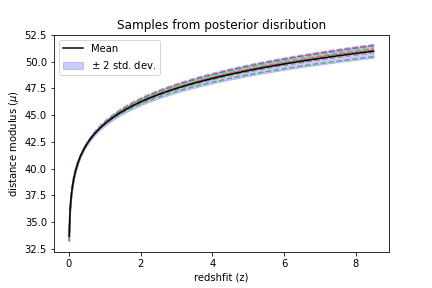
\includegraphics[width=\textwidth]{union/gp/02_Sample_posterior_distibutions.png}
	\caption{Posterior samples drawn from GP}
	\label{fig:posterior_union}
\end{figure}

The error bars with predictions are shown belwo
\begin{figure}[h]
	\centering
	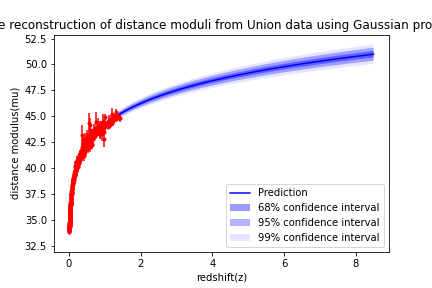
\includegraphics[width=\textwidth]{union/gp/03_Reconstruction_GP.png}
	\caption{Reconstruction from Gaussian Processes}
	\label{fig:gp_re_union}
\end{figure}

Log Marginal Likelihood = -20.3

Score = 99.51
\subsubsection{Testing redshift dependence of luminosity correlations}
\begin{figure}[h]
	\centering
	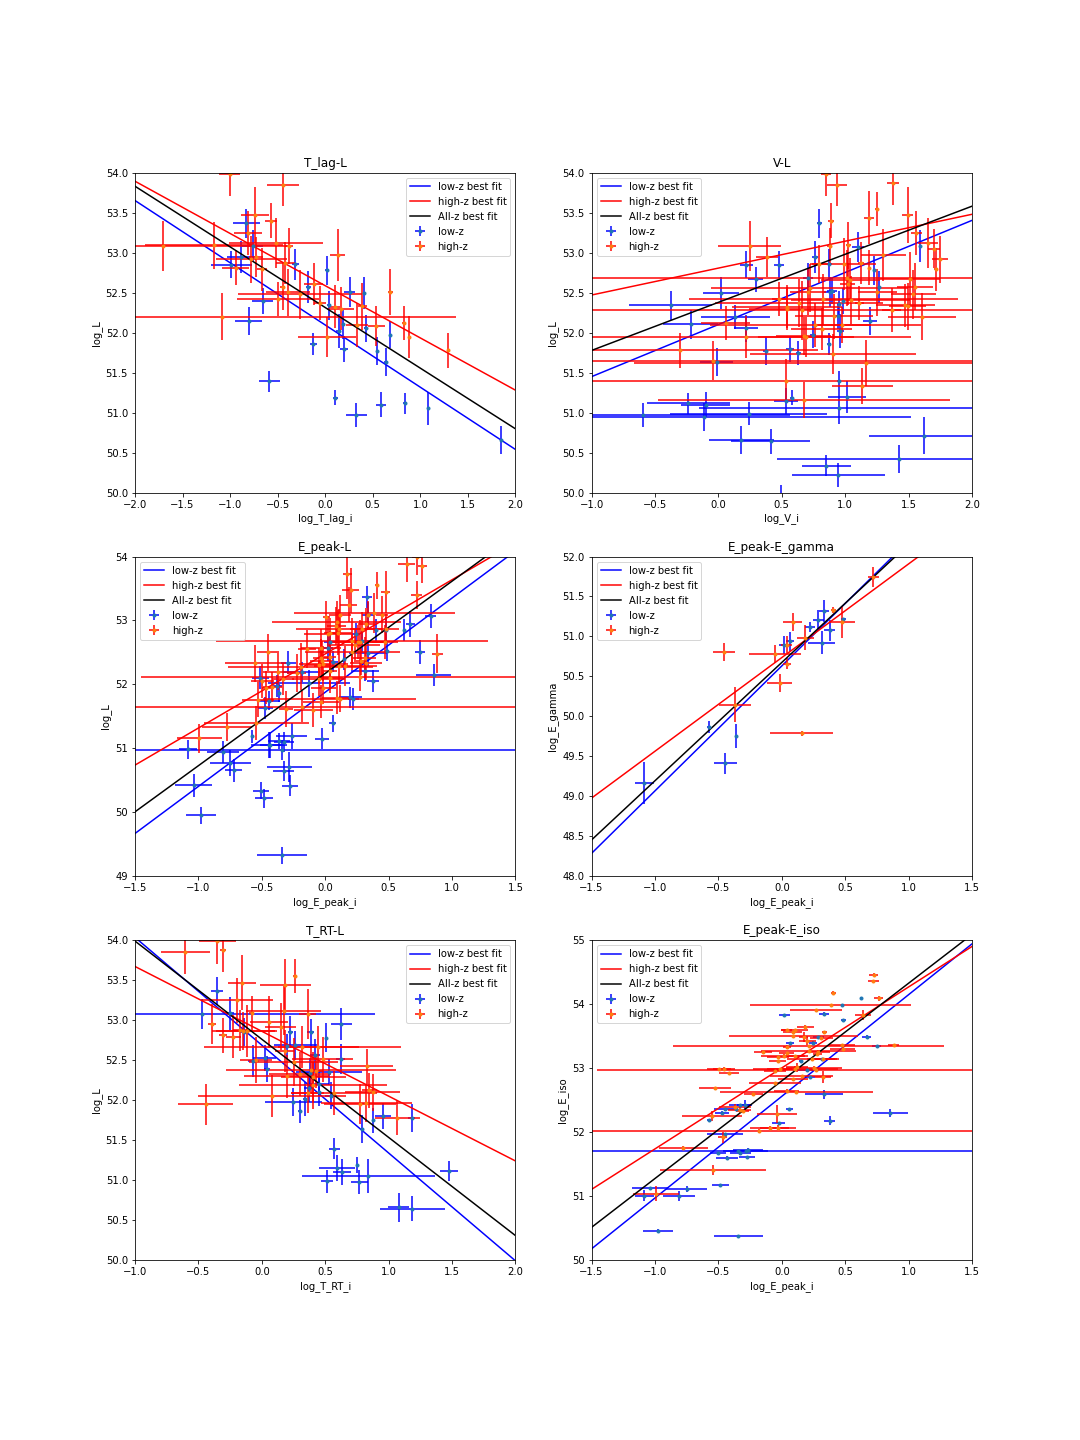
\includegraphics[width=\textwidth]{union/gp/15_correlatin.png}
	\caption{Luminsosity correlations best fit}
	\label{fig:correlation_gp_union}
\end{figure}
\subsubsection{Calibrating distance modulus from $E_{peak}-E_{gamma}$ relation}
\begin{figure}[h]
	\centering
	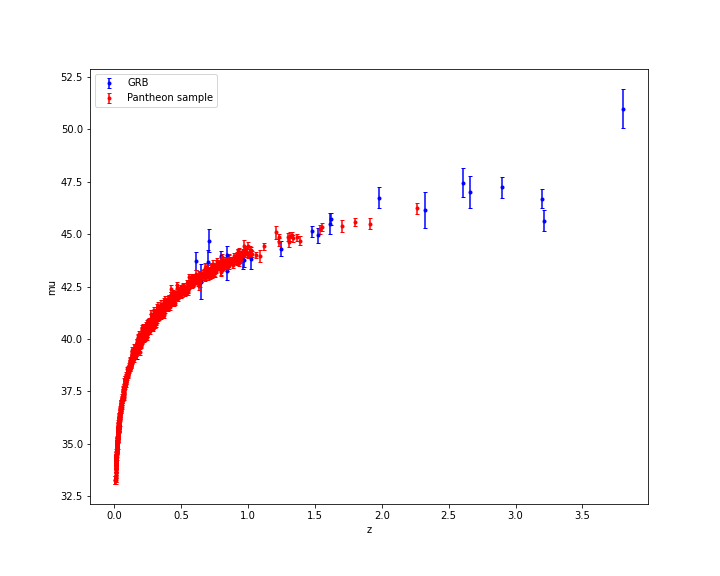
\includegraphics[width=\textwidth]{union/gp/16_GRB_reconstruction.png}
	\caption{GRB Hubble Diagram}
	\label{fig:HD_GRB_GP_union}
\end{figure}
\subsubsection{Constraints on the dark energy}
\begin{figure}[h]
	\centering
	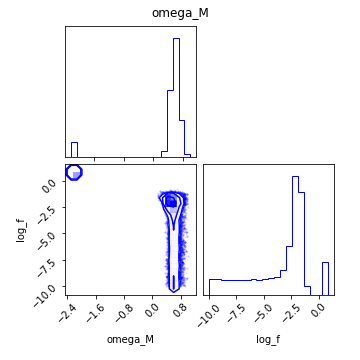
\includegraphics[width=\textwidth]{union/gp/18_omega_M_corner_plot.png}
	\caption{GRB Hubble Diagram}
	\label{fig:OmegaM_GP_union}
\end{figure}
\begin{table}
\centering
\begin{tabular}{|c|c|c|c|c|c|c|c|c|}
\hline
Correlation & sample & N & a & $a_err$ & b & $b_err$ & $\sigma$ & $\sigma_{int}$\\
\hline
\multirow{3}{*}{$T_{lag}-L$} & low-z & 37 & 52.13 & 0.11 & -0.79 & 0.16 & 0.53 & 0.08\\
\cline{2-9}
 & high-z & 32 & 52.62 & 0.07 & -0.65 & 0.12 & 0.36 & 0.06\\
\cline{2-9}
 & All-z & 69 & 52.36 & 0.07 & -0.77 & 0.11 & 0.5 & 0.05\\
\hline
\multirow{3}{*}{$V-L$} & low-z & 47 & 52.11 & 0.25 & 0.65 & 0.37 & 0.93 & 0.14\\
\cline{2-9}
 & high-z & 57 & 52.83 & 0.16 & 0.34 & 0.15 & 0.62 & 0.07\\
\cline{2-9}
 & All-z & 104 & 52.4 & 0.14 & 0.6 & 0.15 & 0.76 & 0.07\\
\hline
\multirow{3}{*}{$E_{peak}-L$} & low-z & 50 & 51.9 & 0.09 & 1.47 & 0.19 & 0.61 & 0.07\\
\cline{2-9}
 & high-z & 66 & 52.52 & 0.06 & 1.13 & 0.15 & 0.41 & 0.04\\
\cline{2-9}
 & All-z & 116 & 52.22 & 0.06 & 1.44 & 0.14 & 0.58 & 0.04\\
\hline
\multirow{3}{*}{$E_{peak}-E_{\gamma}$} & low-z & 12 & 50.65 & 0.08 & 1.56 & 0.19 & 0.24 & 0.09\\
\cline{2-9}
 & high-z & 12 & 50.76 & 0.14 & 1.18 & 0.42 & 0.4 & 0.14\\
\cline{2-9}
 & All-z & 24 & 50.7 & 0.06 & 1.48 & 0.17 & 0.27 & 0.07\\
\hline
\multirow{3}{*}{$T_{RT}-L$} & low-z & 39 & 52.71 & 0.13 & -1.34 & 0.19 & 0.51 & 0.07\\
\cline{2-9}
 & high-z & 40 & 52.9 & 0.08 & -0.83 & 0.18 & 0.43 & 0.06\\
\cline{2-9}
 & All-z & 79 & 52.8 & 0.08 & -1.23 & 0.13 & 0.49 & 0.05\\
\hline
\multirow{3}{*}{$E_{peak}-E_{iso}$} & low-z & 40 & 52.58 & 0.1 & 1.6 & 0.2 & 0.6 & 0.08\\
\cline{2-9}
 & high-z & 61 & 53.03 & 0.06 & 1.28 & 0.14 & 0.39 & 0.04\\
\cline{2-9}
 & All-z & 101 & 52.83 & 0.06 & 1.53 & 0.13 & 0.52 & 0.04\\
\hline
\end{tabular}
\caption{A test caption}
\label{table_gp_union}
\end{table}